\documentclass[12pt]{Qual}
\usepackage{preamble}

\name{Kayla Orlinsky}
\course{Complex Analysis Exam}
\term{Spring 2014}
\hwnum{Spring 2014}

\begin{document}

\begin{problem} $\,$
For $a>0$, evaluate the integral $$\int_0^\infty\frac{\log x}{(a+x)^3},$$ being careful to justify your methods.
\end{problem}


\begin{solution}$\,$
Note that since $x=-a$ on the negative real axis is pole of the function. Namely, ``Ol Faithful'' will intersect a pole in this case.

Thus, we will use the dreaded ``pac man'' contour around the whole plane with the branch cut on the real axis.

\begin{center}
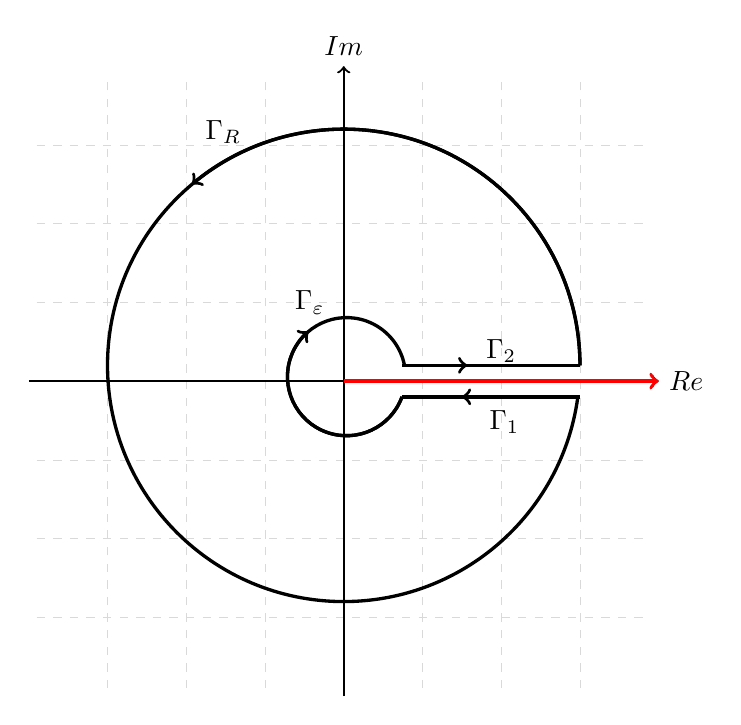
\begin{tikzpicture}
\draw[help lines, color=gray!30, dashed] (-3.9,-3.9) grid (3.9,3.9);
\draw[->,very thick] (3,0.2) arc (0:130:3cm);
\draw[very thick] (3,0.2) arc (0:352:3cm) node[above,yshift=3.1cm,xshift=-4.5cm]{$\Gamma_R$};
\draw[->,very thick] (0.74,-0.2) arc (340:130:0.75cm);
\draw[very thick] (0.74,-0.2) arc (340:12:0.75cm) node[above,yshift=0.5cm,xshift=-1.2cm]{$\Gamma_\varepsilon$};
\draw[->,very thick] (0.74,0.2) -- (1.57,0.2);
\draw[very thick] (0.75,0.2) -- (3,0.2) node[above,yshift=-0.1cm,xshift=-1cm]{$\Gamma_2$};
\draw[->,very thick] (3,-0.2) -- (1.5,-0.2);
\draw[very thick] (3,-0.2) -- (0.74,-0.2) node[above,yshift=-0.6cm,xshift=1.3cm]{$\Gamma_1$};
\draw[->, thick] (-4,0)--(4,0) node[right]{$Re$};
\draw[->, thick] (0,-4)--(0,4) node[above]{$Im$};
\draw[->,very thick,red] (0,0) -- (4,0);
\end{tikzpicture}
\end{center}

Now, we examine $\frac{\log^2z}{(a+z)^3}$ simply because \textbf{Fall 2013: Problem 1} showed that integrating $\log^2z$ inadvertently gave us the value of $\log z$.

Let \begin{align*}
    I_1&=\int_{\Gamma_1}\frac{\log^2 z}{(a+z)^3}dz\\
    I_2&=\int_{\Gamma_2}\frac{\log^2 z}{(a+z)^3}dz\\
    I_\varepsilon&=\int_{\Gamma_\varepsilon}\frac{\log^2 z}{(a+z)^3}dz\\
    I_R&=\int_{\Gamma_R}\frac{\log^2 z}{(a+z)^3}dz
\end{align*}

Note that \begin{align*}
    I_1&=\int_{\Gamma_1}\frac{\log^2 z}{(a+z)^3}dz\\
    &=\int_R^\varepsilon\frac{(\log x+i2\pi)^2}{(a+x)^3}dx\\
    &=\int_R^\varepsilon\frac{\log^2 x+i4\pi\log x-4\pi^2}{(a+x)^3}dx\\
    &=-I_2-i4\pi\int_\varepsilon^R\frac{\log x}{(a+x)^3}dx+4\pi^2\int_\varepsilon^R\frac{1}{(a+x)^3}dx\\
    &=-I_2-i4\pi\int_\varepsilon^R\frac{\log x}{(a+x)^3}dx-4\pi^2\frac{1}{2(a+x)^2}\Big|_\varepsilon^R\\
    &=-I_2-i4\pi\int_\varepsilon^R\frac{\log x}{(a+x)^3}dx-2\pi^2\left[\frac{1}{(a+R)^2}-\frac{1}{(a+\varepsilon)^2}\right]
\end{align*}

Now, \begin{align*}
    |I_R|&=\left|\int_{\Gamma_R}\frac{\log^2z}{(a+z)^3}dz\right|\\
    &\le\int_{\Gamma_R}\frac{|\log^2 z|}{|a+z|^3}d|z|\\
    &\le\int_0^{2\pi}\frac{R|\log R+i\theta|^2}{R^3-a^3}d\theta\\
    &\le 2\pi\frac{R\log^2R}{R^3-a^3}+2\pi\frac{2\pi R}{R^3-a^3}\to0\qquad R\to\infty
\end{align*}

Similarly, \begin{align*}
    |I_\varepsilon|&\le\int_0^{2\pi}\frac{\varepsilon|\log \varepsilon+i\theta|^2}{a^3-\varepsilon^3}d\theta\\
    &\le 2\pi\frac{\varepsilon\log^2\varepsilon}{a^3-\varepsilon^3}+2\pi\frac{2\pi \varepsilon}{a^3-\varepsilon^3}\to0\qquad \varepsilon\to0
\end{align*}

Thus, by the Residue Theorem, \begin{align*}
    2\pi i\res_{z=-a}\frac{\log^2 z}{(a+z)^3}&=2\pi i \frac{1}{2!}\frac{d^2}{dz^2}\log^2z\Big|_{-a}\\
    &=\pi i\frac{d}{dz}\frac{2\log z}{z}\Big|_{-a}\\
    &=2\pi i\left[\frac{1-\log z}{z^2}\right]\Big|_{-a}\\
    &=2\pi i\left[\frac{1-\log(-a)}{a^2}\right]\\
    &=2\pi i\left[\frac{1-\log a-\pi i}{a^2}\right]\\
    &=\lim_{R\to\infty}\lim_{\varepsilon\to 0}(I_1+I_2+I_R+I_\varepsilon)\\
    &=-i4\pi\int_0^\infty\frac{\log x}{(a+x)^3}dx+\frac{2\pi^2}{a^2}\\
    \implies \int_0^\infty\frac{\log x}{(a+x)^3}dx&=\frac{-1}{i2\pi}\left[2\pi i\left[\frac{1-\log a-\pi i}{a^2}\right]-\frac{2\pi^2}{a^2}\right]\\
    &=\frac{\log a-1+\pi i}{2a^2}-\frac{i\pi}{2a^2}\\
    &=\frac{\log a-1}{2a^2}
\end{align*}
\end{solution}
\newpage



\begin{problem} $\,$
Find a conformal mapping of the region $\{z:|z|>1\}\backslash(1,\infty)$ onto the open unit disk $\{z:|z|<1\}.$ You may give your answer as the composition of several mappings, so long as each mapping is precisely described.
\end{problem}

\begin{solution}$\,$
Let \begin{align*}
    T(z)&=\frac{z-i}{z+i}\\
    w_1(z)&=\frac{1}{z}\\
    w_2(z)&=z^{\frac{1}{2}}\qquad\text{branch at }[0,\infty)\\
    w_3(z)&=-z\\
    w_4(z)&=z^2
\end{align*}

\begin{center}
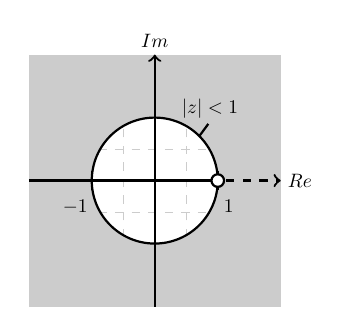
\begin{tikzpicture}[thick,scale=0.4, every node/.style={scale=0.7}]
\fill[gray!40,even odd rule] (-4,-4) rectangle (4,4);
\fill[white,even odd rule] (0,0) circle (2cm);
\draw[help lines, color=gray!40, dashed] (-3.9,-3.9) grid (3.9,3.9);
\draw[thick] (0, 0) circle (2cm) node[above,xshift=1cm,yshift=1cm]{$|z|<1$};
\draw (1.42,1.42) -- (1.7,1.8);
\draw[thick] (2,-0.3) -- (2,0.3) node[below,xshift=0.2cm,yshift=-0.4cm]{$1$};
\draw[->, thick] (-4,0)--(4,0) node[right]{$Re$};
\draw[->, thick] (0,-4)--(0,4) node[above]{$Im$};
\draw[thick] (-2,-0.3) -- (-2,0.3) node[below,xshift=-0.3cm,yshift=-0.4cm]{$-1$};
\draw[gray!40, line width=0.5mm, dashed] (2,0)--(4,0);
 \filldraw[white, draw=black] (2,0) circle (0.2cm);
\end{tikzpicture}
\begin{tikzpicture}
\draw[color=white] (-1,0) rectangle (0.5,1);
\draw[thick,->] (-1,2) -- (0,2) node[above,xshift=-0.5cm]{$w_1$};
\end{tikzpicture}
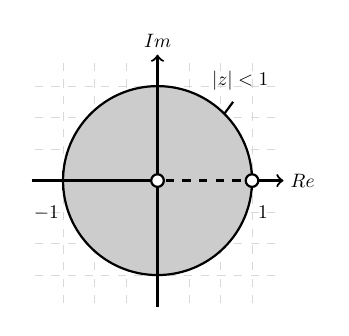
\begin{tikzpicture}[thick,scale=0.4, every node/.style={scale=0.7}]
\draw[help lines, color=gray!30, dashed] (-3.9,-3.9) grid (3.9,3.9);
\draw (2.12,2.12) -- (2.4,2.5);
 \fill[gray!40,even odd rule, dashed] (0,0) circle (3cm);
   \draw (0, 0) circle (3cm) node[above,xshift=1.5cm,yshift=1.5cm]{$|z|<1$};
\draw[thick] (3,-0.3) -- (3,0.3) node[below,xshift=0.2cm,yshift=-0.5cm]{$1$};
\draw[->, thick] (-4,0)--(4,0) node[right]{$Re$};
\draw[->, thick] (0,-4)--(0,4) node[above]{$Im$};
\draw[thick] (-3,-0.3) -- (-3,0.3) node[below,xshift=-0.3cm,yshift=-0.5cm]{$-1$};
\draw[gray!40, line width=0.5mm, dashed] (0,0)--(3,0);
 \filldraw[white, draw=black] (0,0) circle (0.2cm);
 \filldraw[white, draw=black] (3,0) circle (0.2cm);
\end{tikzpicture}
\begin{tikzpicture}
\draw[color=white] (-1,0) rectangle (0.5,1);
\draw[thick,->] (-1,2) -- (0,2) node[above,xshift=-0.5cm]{$w_2$};
\end{tikzpicture}
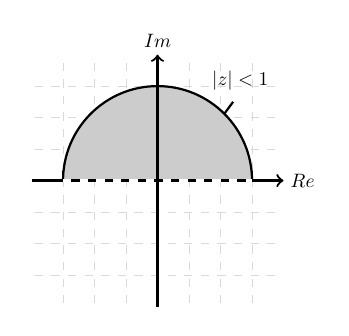
\begin{tikzpicture}[thick,scale=0.4, every node/.style={scale=0.7}]
\draw[help lines, color=gray!30, dashed] (-3.9,-3.9) grid (3.9,3.9);
\draw (2.12,2.12) -- (2.4,2.5);
\fill[gray!40,even odd rule, dashed] (0,0) circle (3cm);
\draw (0, 0) circle (3cm) node[above,xshift=1.5cm,yshift=1.5cm]{$|z|<1$};
\draw[thick] (3,-0.3) -- (3,0.3) node[below,xshift=0.2cm,yshift=-0.5cm]{$1$};
\draw[thick] (-3,-0.3) -- (-3,0.3) node[below,xshift=-0.3cm,yshift=-0.5cm]{$-1$};
\fill[white] (-4,-4) rectangle (4,0);
\draw[help lines, color=gray!30, dashed] (-3.9,-3.9) grid (3.9,0);
\draw[->, thick] (-4,0)--(4,0) node[right]{$Re$};
\draw[->, thick] (0,-4)--(0,4) node[above]{$Im$};
\draw[white,line width=0.4mm, dashed] (-3,0)--(3,0);
\end{tikzpicture}

\begin{tikzpicture}%[thick,scale=0.5, every node/.style={scale=0.6}]
\draw[thick,->] plot [smooth] coordinates {(3,0.6) (3,0) (-10,0) (-11,-1)} node[above,xshift=7cm,yshift=1cm]{$w_3$};
\end{tikzpicture}

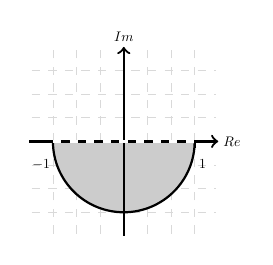
\begin{tikzpicture}[thick,scale=0.3, every node/.style={scale=0.5}]
\draw[help lines, color=gray!30, dashed] (-3.9,-3.9) grid (3.9,3.9);
\draw (2.12,2.12) -- (2.4,2.5);
 \fill[gray!40,even odd rule, dashed] (0,0) circle (3cm);
   \draw (0, 0) circle (3cm);
\draw[thick] (3,-0.3) -- (3,0.3) node[below,xshift=0.2cm,yshift=-0.5cm]{$1$};
\draw[thick] (-3,-0.3) -- (-3,0.3) node[below,xshift=-0.3cm,yshift=-0.5cm]{$-1$};
\fill[white] (-4,4) rectangle (4,0);
\draw[help lines, color=gray!30, dashed] (-3.9,3.9) grid (3.9,0);
\draw[->, thick] (-4,0)--(4,0) node[right]{$Re$};
\draw[->, thick] (0,-4)--(0,4) node[above]{$Im$};
\draw[white,line width=0.4mm, dashed] (-3,0)--(3,0);
\end{tikzpicture}
\begin{tikzpicture}
\draw[color=white] (-1,0) rectangle (0.5,1);
\draw[thick,->] (-1,2) -- (0,2) node[above,xshift=-0.5cm]{$T^{-1}$};
\end{tikzpicture}
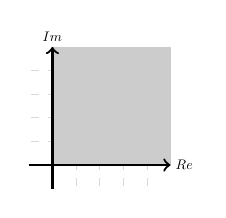
\begin{tikzpicture}[thick,scale=0.3, every node/.style={scale=0.5}]
\draw[help lines, color=gray!30, dashed] (-0.9,-0.9) grid (4.9,4.9);
 \fill[gray!40,even odd rule] (0,0) rectangle (5,5);
\draw[->, thick] (-1,0)--(5,0) node[right]{$Re$};
\draw[->, thick] (0,-1)--(0,5) node[above]{$Im$};
\end{tikzpicture}
\begin{tikzpicture}
\draw[color=white] (-1,0) rectangle (0.5,1);
\draw[thick,->] (-1,2) -- (0,2) node[above,xshift=-0.5cm]{$w_4$};
\end{tikzpicture}
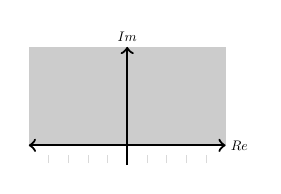
\begin{tikzpicture}[thick,scale=0.25, every node/.style={scale=0.5}]
\draw[help lines, color=gray!30, dashed] (-4.9,-0.9) grid (4.9,4.9);
 \fill[gray!40,even odd rule] (-5,0) rectangle (5,5);
\draw[<->, thick] (-5,0)--(5,0) node[right]{$Re$};
\draw[->, thick] (0,-1)--(0,5) node[above]{$Im$};
\end{tikzpicture}
\begin{tikzpicture}
\draw[color=white] (-1,0) rectangle (0.5,1);
\draw[thick,->] (-1,2) -- (0,2) node[above,xshift=-0.5cm]{$T$};
\end{tikzpicture}
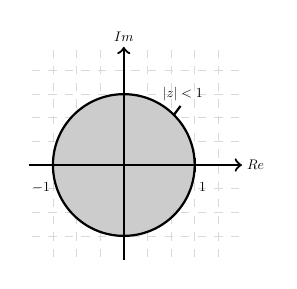
\begin{tikzpicture}[thick,scale=0.3, every node/.style={scale=0.5}]
\draw[help lines, color=gray!30, dashed] (-3.9,-3.9) grid (4.9,4.9);
\draw (2.12,2.12) -- (2.4,2.5);
 \fill[gray!40,even odd rule, dashed] (0,0) circle (3cm);
   \draw (0, 0) circle (3cm) node[above,xshift=1.5cm,yshift=1.5cm]{$|z|<1$};
\draw[thick] (3,-0.3) -- (3,0.3) node[below,xshift=0.2cm,yshift=-0.5cm]{$1$};
\draw[->, thick] (-4,0)--(5,0) node[right]{$Re$};
\draw[->, thick] (0,-4)--(0,5) node[above]{$Im$};
\draw[thick] (-3,-0.3) -- (-3,0.3) node[below,xshift=-0.3cm,yshift=-0.5cm]{$-1$};
\end{tikzpicture}
\end{center}
\end{solution}
\newpage




\begin{problem} $\,$
Suppose that $f_n$ are analytic functions on a connected open set $U\subset\mathbb{C}$ and that $f_n\to f$ uniformly on compact subsets of $U$. In each case indicate the main setps in the proofs of the following stnadard results.
\begin{enumerate}[label=(\alph*)]
    \item $f$ is analytic in $U;$
    \item $f_n'\to f'$ uniformly on compact subsets of $U;$
    \item if $f_n(z)\not=0$ for all $n$ and all $z\in U$, then either $f(z)\not=0$ for all $z\in U$ or else $f\equiv 0$.
\end{enumerate}
\end{problem}


\begin{solution}$\,$
\textit{\textbf{What a poorly worded question... what are ``main steps''?}}

\begin{enumerate}[label=(\alph*)]
    \item Let $\varepsilon>0$. Then, there exists an $N$ such that $|f_n(z)-f(z)|<\varepsilon$ for all $n\ge N$ and all $z\in K\text{ compact }\subset U$.

    Clearly this forces any singularities of $f$ to be isolated. Else uniform convergene via analytic functions is not possible.

    Furthermore, if $f$ has a removable singularity at $z_0\in K$, then $f(z_0)=w$ but $\lim_{z\to z_0}f(z)=w'=\lim_{n\to\infty}f_n(z_0)$, so uniform convergence is not possible unless $w'=w$, namely $f$ cannot have a removable singularity.

    Similarly, if $f$ has a pole or essential singularity in $K$, then again this will contradict uniform convergence. So $f$ is analytic in all compact subsets of $U$. Namely, $f$ is analytic in $U.$
    \item Let $K\subset U$ be compact. Let $z\in K$ and $\rho$ such that $B_\rho(z)\subset K$. Then let $\varepsilon>0$ and $N$ such that $|f_n(z)-f(z)|<\varepsilon$ for all $n\ge N$ and all $z\in K$. Then \begin{align*}
        \left|f_n'(z)-f'(z)\right|&=\left|\int_{|\xi-z|=\rho}\frac{f_n(\xi)}{(\xi-z)^2}d\xi-\int_{|\xi-z|=\rho}\frac{f(\xi)}{(\xi-z)^2}d\xi\right|\\
        &=\left|\int_{|\xi-z|=\rho}\frac{f_n(\xi)-f(\xi)}{(\xi-z)^2}d\xi\right|\\
        &\le\int_{|\xi-z|=\rho}\frac{|f_n(\xi)-f(\xi)|}{|\xi-z|}d|\xi|\\
        &\le\int_0^{2\pi}\frac{\varepsilon}{\rho}d\theta\\
        &=\frac{2\pi\varepsilon}{\rho}
    \end{align*}

    for all $n\ge N$ and so $f_n'\to f$ for all $z\in K$.

    \item Let $f(z)=0$ for some $z$. Let $\rho>0$ be such that $B_\rho(z)$ contains only one zero of $f$, namely $z$ itself. Then from (b), $f_n'\to f'$, so \begin{align*}
        0&=\text{ Number of zeros of }f_n\text{ in }B_\rho(z)\\
        &=\frac{1}{2\pi i}\int_{|\xi-z|=\rho}\frac{f_n(\xi)}{f_n'(\xi)}d\xi\to\frac{1}{2\pi i}\int_{|\xi-z|=\rho}\frac{f(\xi)}{f'(\xi)}d\xi\\
        &=\text{ Number of zeros of }f\text{ in }B_\rho(z)\\
        &=1
    \end{align*} a contradiction unless $f\equiv 0$ in which case, $$\frac{1}{2\pi i}\int_{|\xi-z|=\rho}\frac{f_n(\xi)}{f_n'(\xi)}d\xi\to0.$$
\end{enumerate}
\end{solution}
\newpage





\begin{problem} $\,$
\begin{enumerate}[label=(\alph*)]
    \item Suppose that $f$ is analytic on the open unit disk $\{z:|z|<1\}$ and that there exists a constant $M$ such that $|f^k(0)|\le k^4M^k$ for all $k\ge 0.$ Show that $f$ can be extended to be analytic on $\mathbb{C}.$
    \item Suppose that $f$ is analytic on the open unit disk $\{z:|z|<1\}$ and that there exists a cosntant $M>1$ such that $|f(1/k)|\le M^{-k}$ for all $k\ge1$. Show that $f$ is identically zero.
\end{enumerate}
\end{problem}


\begin{solution}$\,$
\begin{enumerate}[label=(\alph*)]
    \item Note that this forces $f(0)=0$ and so the statement as written, makes no sense since $f^k(0)=0$ for all $k.$

    Thus, $|f^{(k)}(0)|\le k^4M^k$ for all $k\ge0.$

    We can write a Taylor Series for $f$ inside the disk.

    $$f(z)=\sum_{n=0}^\infty\frac{f^{(n)}(0)}{n!}z^n.$$ Now, for arbitrary $z\in\mathbb{C}$, \begin{align*}
        |f(z)|&\le\sum_{n=0}^\infty\frac{|f^{(n)}(0)|}{n!}|z|^n\\
        &\le\sum_{n=0}^\infty\frac{n^4M^n}{n!}|z|^n\\
        &=\sum_{n=0}^\infty\frac{n^4 R^n}{n!}\qquad R=M|z|
    \end{align*}

    This is a real sum, and we can check that it converges by ratio test. Namely, $\sum_{n=0}^\infty a_n$ converges absolutely if $$\lim_{n\to\infty}\frac{|a_{n+1}|}{|a_n|}<1$$ \begin{align*}
        \lim_{n\to\infty}\frac{a_{n+1}}{a_n}&=\lim_{n\to\infty}\frac{\frac{(n+1)^4 R^{n+1}}{(n+1)!}}{\frac{n^4 R^n}{n!}}\\
        &=\lim_{n\to\infty}\frac{(n+1)^4 R^{n+1} n!}{(n+1)!n^4 R^n}\\
        &=\lim_{n\to\infty}\frac{(n+1)^4 R}{n^4(n+1)}\\
        &=\lim_{n\to\infty}\frac{(n+1)^3 R}{n^4}=0
    \end{align*}

    Thus, the series absolutely converges. Furthermore, for all $|z|<\frac{R}{M}$, convergence is clearly uniform and since $R$ is arbitrary, we get that $f$ can be extended analytically to all of $\mathbb{C}$.

    \item Suppose that $f$ is analytic on the open unit disk $\{z:|z|<1\}$ and that there exists a constant $M>1$ such that $|f(1/k)|\le M^{-k}$ for all $k\ge1$.

    This gives that $f(0)=0$. Assume $f$ is non-constant. Then we can write $f(z)=z^ng(z)$ where $g$ is analytic and nonzero at $0$.

    Then $$|f(1/k)|=\frac{|g(1/k)|}{k^n}\le\frac{1}{M^k}.$$

    Namely, $$\lim_{k\to\infty}|g(1/k)|\le\lim_{k\to\infty}\frac{k^n}{M^k}=0$$ by induction.

    This contradicts that $g$ is nonzero at $0$ and so $g$ cannot exist. Namely, $f$ cannot exist and must therefore be constant.

    Since $f(0)=0$, $f\equiv 0.$
\end{enumerate}
\end{solution}


\end{document}
